\documentclass[oneside]{book}
\usepackage{apjfonts}
\usepackage{geometry}
\usepackage{graphicx}
\usepackage{titletoc, titlesec}
\usepackage{hyperref}
\usepackage{geometry}
\usepackage{color, framed}
\usepackage{amsmath,mathrsfs,amsfonts}
\usepackage{natbib}

\definecolor{main}{RGB}{0,120,2}%
\definecolor{seco}{RGB}{230,90,7}%
\definecolor{thid}{RGB}{0,160,152}%

\definecolor{shadecolor}{rgb}{0.92,0.92,0.92}

\hypersetup{
 breaklinks,
 unicode,                
 bookmarksnumbered  =true,
 bookmarksopen      =true, 
 pdfsubject         =\@author \@title Book,
 pdfkeywords        ={ElegantBook},
 pdfcreator         ={XeLaTeX with ElegantBook class},
 colorlinks,
 linkcolor          =main,
 plainpages         =false,
 pdfstartview       =FitH,
 pdfborder={0 0 0},
 linktocpage
 }


\geometry{
    a4paper,
   left=27mm,  %% or inner=23mm
   right=27mm, %% or outer=18mm
   top=25.4mm, bottom=25.4mm,
   headheight=2.17cm,
   headsep=4mm,
   footskip=12mm
}

\titleformat{\chapter}[hang]{\Huge\bfseries}{Chapter \thechapter}{1cm}{}[]

\DeclareMathAlphabet{\mathbi}{OT1}{cmr}{bx}{it}
\SetMathAlphabet\mathbi{bold}{OT1}{cmr}{bx}{it}

\def\brains{{\texttt{brains}}}

\begin{document}

\title{\bf BRAINS:\\
Bayesian Reverberation-mapping Analysis Integrated
with Nested Sampling}
\author{Yan-Rong Li\\
Institute of High Energy Physics}

\maketitle
\tableofcontents
\mainmatter

\clearpage
\newpage

\vspace*{10cm}
{\Huge\centerline{\bf Part I: Users' Guide}}


\chapter{Installation}
\section{Third-Party Packages}
{\brains} requires the following third-party packages:
\begin{itemize}
 \item {\bf GSL}. GSL is used to generate random numbers, perform interpolation, and calculate some special functions. GSL is available at 
 \url{https://www.gnu.org/software/gsl}.
 
 \item {\bf FFTW}. FFTW is used to implement Gaussian smoothing on the line profiles. FFTW is available at \url{http://fftw.org}.
 
 \item {\bf LAPACK}. LAPACK is used to perform numerical linear algebra calculations, such as matrix operations and Cholesky decomposition.
 LAPACK is a fortran library. Its C interface is LAPACKE, included in the LAPACK package. One needs to configure the LAPACK installation
 options to switch on LAPACKE. LAPACK is available at \url{https://netlib.sandia.gov/lapack}.
 
 \item {\bf MPICH}. MPICH is a high performace and widely portable implementation of the Message Passing Interface standard.
 MPICH is available at \url{http://www.mpich.org}. 
 
 \item {\bf DNest}. DNest is a library to implement diffusive nested sampling. DNest is available at \url{https://github.com/LiyrAstroph/DNest_C}.
\end{itemize}
In popular Linux distributions, one can use the system package manager to install the above packages, except for DNest. For example, in Fedora distribution, 
the corresponding terminal commands are 
\begin{verbatim}
 sudo dnf install gsl fftw3 lapack mpich
\end{verbatim} 

\section{Configure the \texttt{Makefile}}
To compile {\brains}, one needs first to proporiately configure the \texttt{Makefile}. In Linux systems, typical configurations look like
\begin{shaded}
\scriptsize
\begin{verbatim}
ifeq ($(SYSTEM), "Linux")
GSL_INCL    = $(shell pkg-config --cflags gsl)
GSL_LIBS    = $(shell pkg-config --libs gsl) 

LAPACK_INCL = -I/usr/include/lapacke
LAPACK_LIBS = -L/usr/lib64 -llapacke -llapack -lblas

DNEST_INCL  = -I /home/liyropt/Projects/GIT/DNest/
DNEST_LIBS  = -L /home/liyropt/Projects/GIT/DNest -ldnest

FFTW_INCL   = $(shell pkg-config --cflags fftw3) 
FFTW_LIBS   = $(shell pkg-config --libs fftw3) 

MPICHINCL     = $(shell pkg-config --cflags mpich) 
MPICHLIB    = $(shell pkg-config --libs mpich) 
endif
\end{verbatim}
\end{shaded}
Change the values of the variables in line with your system's configurations.

\section{Compiling}
The command for compiling is 
\begin{verbatim}
 make
\end{verbatim}
This will create an executable file `` \texttt{brains}'' in the local directory.


\chapter{Running}

\section{Running Commands}
First change the directory to where \texttt{brains} is installed. To run \texttt{brains}, one can use command
\begin{verbatim}
brains [FILE] [OPTION]
\end{verbatim}
or
\begin{verbatim}
mpiexec [MPI_OPTION] brains [FILE] [OPTION]
\end{verbatim}
where \texttt{[FILE]} is the name of parameter file, \texttt{[MPI\_OPTION]} is the options for MPI and \texttt{[OPTION]}
is the command-line options for \texttt{brains}. For example, to run \texttt{brains} with 3 cores, use
\begin{verbatim}
mpiexec -n 3 brains param
\end{verbatim}
where \texttt{param} is the parameter file. 

\texttt{brains} recognizes following command-line options:
\begin{shaded}
\scriptsize
\begin{verbatim}
    -h
        print help information.
    -p
        only do posterior processing.
    -r
        restart from the backup.
    -t
        specify tempering temperature in posterior processing.
    -s 
        set a seed for the random number generator.
    -c
        only do posterior processing and recalculate the posterior sample information.
    -e
        examine the priors.
\end{verbatim}
\end{shaded}


\section{Parameter File}
A typical paramete file looks like
\begin{shaded}
\scriptsize
\begin{verbatim}
% parameter file
% lines beginning with '%' are regarded as comments and are neglected
% 

FileDir                     /home/liyropt/Projects/GIT/BRAINS     

FlagDim                     2                         

FlagBLRModel                6                           
       
%========================================================================
% data file

ContinuumFile               data/sim_con.txt          
LineFile                    data/sim_hb.txt          
Line2DFile                  data/sim_hb2d.txt        

%========================================================================
% reconstruction
NConRecon                   200                         
FlagTrend                   0                           
FlagTrendDiff               0                            
ConConstructFileOut         data/pcon.txt              

FlagFixVar                  0                           
NLineRecon                  100                         
LineConstructFileOut        data/pline.txt              
TranFileOut                 data/tran.txt               

NVelRecon                   42                          
Line2DConstructFileOut      data/pline2d.txt            
Line2DDataConstructFileOut  data/pline2d_data.txt       
Tran2DFileOut               data/tran2d.txt             
Tran2DDataFileOut           data/tran2d_data.txt       

NCloudPerCore               5000                        
NVPerCloud                  5                           

NTau                        200                         
RCloudMax                   -1                         
TimeBack                    -1                          

FlagCloudsOut               1                           
CloudsFileOut               data/clouds.txt             

%========================================================================
%
FlagCloudsForceUpdate       1                           

FlagConSysErr               0                           
FlagLineSysErr              0                           

%========================================================================
% spectral broadening

InstRes                     220                         
                                                         

InstResErr                  34.0                          

InstResFile                 data/arp151_broaden.txt       
                                                          
%========================================================================
% narrow-line component
% use a gaussian to model the narrow-line component

FlagNarrowLine              0                                                                               

FluxNarrowLine              1.5                        
FluxNarrowLineErr           0.50                        
WidthNarrowLine             14.0                        
WidthNarrowLineErr          4.4                         
ShiftNarrowLine             10.0                         
ShiftNarrowLineErr          0.0                        

%========================================================================
% 
FlagLineCenter              1
LineCenterErr               62.0                        

%========================================================================
% set fixed BLR parameters and their fixed values
% do not put sapce in the strings
% 1: fixed; 0: not fixed;
% values are separated by ":"

BLRParFix                   0000000000
BLRParFixVal                0.0:1.0           
\end{verbatim}
\end{shaded}

In parameter file, lines beginning with '\%' are regarded as comments and are neglected, so that you can freely add
comments for your convinence as in the above example. Also, the orders of parameters can be changed freely. Most
of the parameters are given a name that largely indicates the corresponding meanings.


\section{OPTION File for DNest}
The format of option file for DNest looks like as follows,
\begin{shaded}
\scriptsize
\begin{verbatim}
# File containing parameters for DNest
# Put comments at the top, or at the end of the line.
# Do not change the order of lines.
# Lines beginning with '#' are regarded as comments.

2	    # Number of particles
2000	# new level interval
2000	# save interval
100	  # threadSteps - how many steps each thread should do independently before communication
20	  # maximum number of levels
10	  # Backtracking scale length (lambda in the paper)
100	  # Strength of effect to force histogram to equal push. 0-10 is best. (beta in the paper)
1000	  # Maximum number of saves (0 = infinite)
data/sample.txt                 # sample file
data/sample_info.txt            # sample_info file
data/levels.txt                 # level file
data/sampler_state.txt          # sample state file
data/posterior_sample.txt       # posterior sample file
data/posterior_sample_info.txt  # posterior sample info file
data/limits.txt                 # limits file
\end{verbatim}
\end{shaded}

The option file for continuum reconstruction is \texttt{OPTIONSCON}, for 1d RM is \texttt{OPTIONS1D}, and 
for 2d RM is \texttt{OPTIONS2D}. \texttt{brains} will automatically read these options appropriately. 

One should not change the orders of lines. Lines beginning with '\#' are regarded as comments. 
There is not a general rule to set the values of options. The most important options are the options 
for new level interval and maximum number of levels. Sufficently large values will work better, but also
will cause extra computation time. The option for maximum number of saves controls the length of the 
Markov chains. Note that this is not the length of the final posterior sample. 

To check whether the values of options are appropriate, one may run the python script \texttt{postprocess.py}
in the subdirectory to inspect the log-likelihood-curve (\citealt{Brewer2011}); see also the user mannual in the 
package DNest3 developed by Brendon J. Brewer, which is available at \url{https://github.com/eggplantbren/DNest3}. 

\begin{figure}[hp]
\centering 
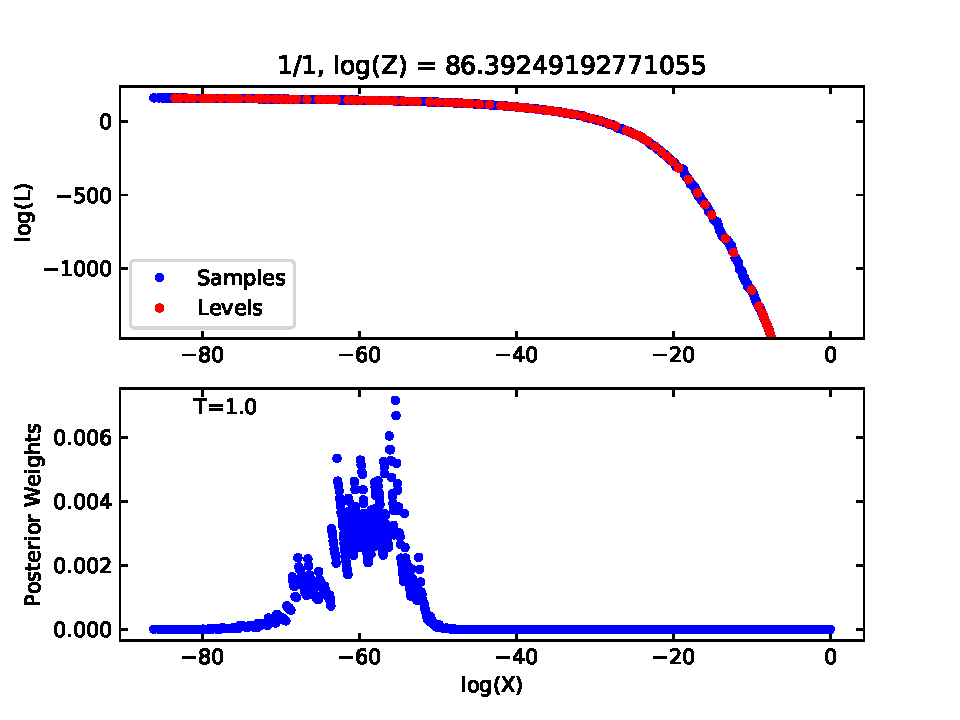
\includegraphics[width=0.45\textwidth]{post1.pdf}
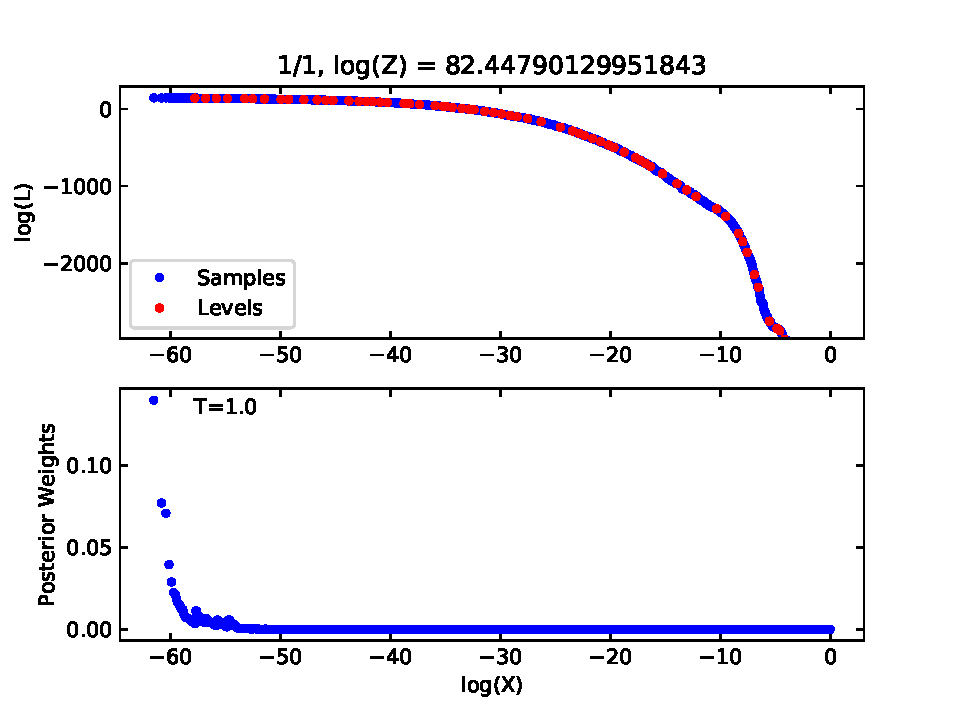
\includegraphics[width=0.45\textwidth]{post2.pdf}
\caption{Examples for log-likelihood cruve: (left) a good run with sufficiently appropriate options and (right) a bad 
run with inappropriate options.}
\end{figure}


\begin{thebibliography}{10}
\bibitem[Li et al.(2018)]{Li2018}
  Li, Y.-R., Songsheng, Y.-Y., Qiu, J. et al. 2018, ApJ in press (arXiv: 1811.06302)
\bibitem[Brewer \& Foreman-Mackey(2016)]{Brewer2016}
  Brewer, B. J. \& Foreman-Mackey, D. 2016, Journal of Statistical Software, 86, 1297 (arXiv:1606.03757)
\bibitem[Brewer et al.(2011)]{Brewer2011}
  Brewer, B., J. et al., 2011, Statistics and Computing, 21, 649 (arXiv: 0912.2380)
\end{thebibliography}

\clearpage
\newpage

\vspace*{10cm}
{\Huge\centerline{\bf Part II: Broad-Line Region Modeling}}


\chapter{BLR Modeling}

\section{Coordinate rotation}
\begin{figure}[h!]
\centering
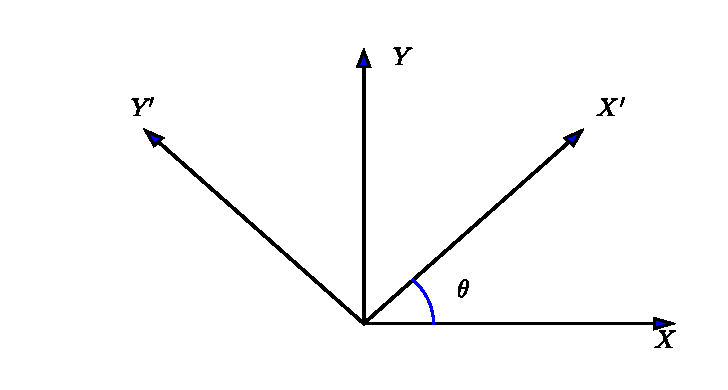
\includegraphics[width=0.5\textwidth]{coord.pdf}
\end{figure}

For the rotation of a coordinate (XOY) by an angle of $\theta$ to (X'OY'), there are relations
\begin{equation}
\left[\begin{array}{c}
\mathbi{e}_{x'} \\
\mathbi{e}_{y'}
\end{array}\right]=\left[\begin{array}{cc}
\cos\theta & \sin \theta  \\
-\sin\theta &  \cos \theta       
\end{array}\right]\left[\begin{array}{c}
\mathbi{e}_{x} \\
\mathbi{e}_{y}
\end{array}\right].
\end{equation}
and 
\begin{equation}
\left[\begin{array}{c}
\mathbi{e}_{x} \\
\mathbi{e}_{y}
\end{array}\right]=\left[\begin{array}{cc}
\cos\theta & -\sin \theta  \\
\sin\theta &  \cos \theta       
\end{array}\right]\left[\begin{array}{c}
\mathbi{e}_{x'} \\
\mathbi{e}_{y'}
\end{array}\right].
\end{equation}
Therefore, for a vector $A$, its components in (XOY) and (X'OY') are related by
\begin{equation}
A=[x', y'] \left[\begin{array}{c}
\mathbi{e}_{x'} \\
\mathbi{e}_{y'}
\end{array}\right] = [x, y]\left[\begin{array}{c}
\mathbi{e}_{x} \\
\mathbi{e}_{y}
\end{array}\right]=[x, y] \left[\begin{array}{cc}
\cos\theta & -\sin \theta  \\
\sin\theta &  \cos \theta       
\end{array}\right]\left[\begin{array}{c}
\mathbi{e}_{x'} \\
\mathbi{e}_{y'}
\end{array}\right].
\end{equation}
This yields
\begin{equation}
\left[\begin{array}{c}
x' \\
y'
\end{array}\right]=\left[\begin{array}{cc}
\cos\theta & \sin \theta  \\
-\sin\theta &  \cos \theta       
\end{array}\right]\left[\begin{array}{c}
x \\
y
\end{array}\right].
\end{equation}


In right-handed coordinate frame, we perform a rotation around $y$-axis by an angle of $l_\theta$ and 
then a rotation around $z$-axis by an angle of $l_\phi$. The transformation matrix is
\begin{equation}
\left[\begin{array}{ccc}
\cos l_\phi & \sin l_\phi & 0 \\
-\sin l_\phi &  \cos l_\phi & 0 \\
     0      &      0       & 1 
\end{array}\right]
\left[\begin{array}{ccc}
\cos l_\theta  & 0  & -\sin l_\theta\\
   0      &      1        &  0  \\
\sin l_\theta &  0  & \cos l_\theta 
\end{array}\right]=
\left[\begin{array}{ccc}
\cos l_\phi\cos l_\theta  & \sin l_\phi  & -\cos l_\phi\sin l_\theta\\
-\sin l_\phi\cos l_\theta      & \cos l_\phi        &  \sin l_\phi\sin l_\theta  \\
\sin l_\theta &  0  & \cos l_\theta 
\end{array}\right]
.
\end{equation}

\section{Time Lag}
The obsever is located at $(D\rightarrow\infty, 0, 0)$, i.e., the line of sight is along $x-$axis. 
For a cloud at $(x, y, z)$, its time lag is
\begin{equation}
\tau =\sqrt{x^2+y^2+z^2} + \sqrt{(D-x)^2+y^2+z^2} - D \approx r + D(1-x/D) - D \approx r - x,
\end{equation}
where $r=\sqrt{x^2+y^2+z^2}$.

The angle between the line of sight and the line of cloud is
\begin{equation}
 \cos \varphi = \frac{D\cdot x}{D\cdot r} = \frac{x}{r}.
\end{equation}

{\bf waiting for update...}
\end{document}

